\chapter{Methodology}

\section{Introduction}

In order to characterise the synthesised materials and acquire information about the chemistry, crystallinity, morphology as well as its optical and electrical properties a suite of state of the art techniques has to be utilised. An overview of those techniques has been provided in theory and experimental setup.

\section{Raman spectroscopy}

Raman spectroscopy is one of the most useful and versatile characterisation techniques for 2D TMDCs due to its non destructive and ease of use. The lack of need to extensively prepare the sample like in some other techniques allows for relatively fast measurements of a large number of samples. Additionally the lack of transfer required results in minimal changes to to the material itself as well allows for easier tracking of specific areas of the sample across different techniques. Raman spectroscopy can be used to measure as grown by CVD samples on $Si/SiO_2$ substrate or any other solid substrate as well as liquid solution samples produced by liquid exfoliation.

The Raman spectroscopy can be used to extract information about the chemistry of the material as well as the crystal structure, the number of layers of 2D TMDCs or the strain within the layers. 

When a material is irradiated with light the photons generally scatter at different angle but same wavelength. However certain small part of the incident photons (about 1 in 10 million) is scattered at different wavelength than the incident one. This is known as the Raman effect and the photons that are scattered at wavelengths greater than the incident ones are due to Stokes scattering, while the ones emitted at wavelengths smaller than the incident one are due to anti-Stokes scattering. In the Stokes scattering phenomena the phonon is emitted while during the anti-Stokes scattering the phonon is absorbed as seen in Figure \ref{fig:MethodologyRamanEnergyLevels}. In order for the Raman effect to take place a transition between two resonant states must occur. The probability of transition from lower to higher energy state depends on the population of the states. In a thermodynamically stable system the lower energy states are more occupied than the higher energy and therefore the transition from lower to higher is more likely to occur (Stokes scattering). The spectrum of photons scattered as a result of Raman scattering forms what is known as Raman spectrum, where the number of photons scattered is plotted against the photon frequency difference between the incident and the scattered photons. The spectrum is symmetrical around the spectrum origin in regards to the frequency but not in terms of intensity. Because of that only the Stokes part is generally used as a Raman spectrum.

\begin{figure}[!ht]
	\begin{center}
		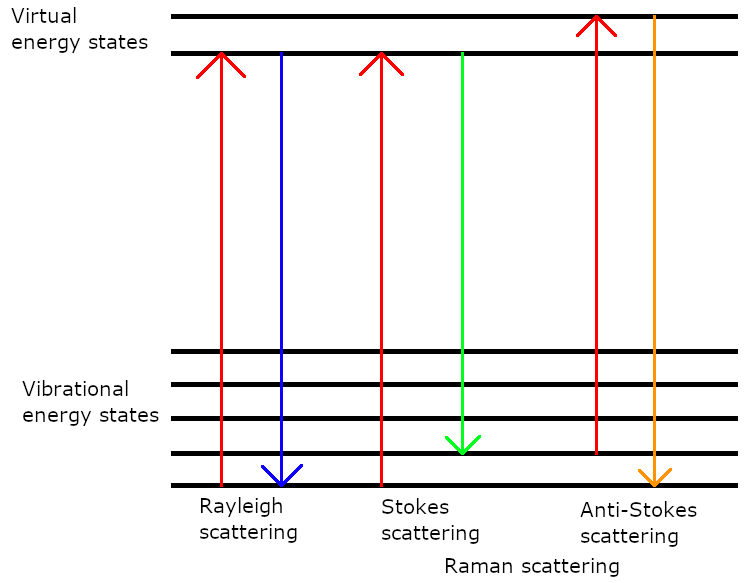
\includegraphics[scale=0.3]{Methodology/RamanEnergyLevels.png}
		\caption{An energy diagram comparing elastic and inelastic scattering. Reproduced from en.wikipedia.org}
		\label{fig:MethodologyRamanEnergyLevels}
	\end{center}
\end{figure}

The phonons that are emitted or absorbed during the transitions between the virtual states in the Raman effect are phonons of the vibrational modes in the material. For any solid state crystalline material the point group can be defined. Using the point group the available vibrational modes can be found. In order for Raman scattering to occur a change in polarisability must occur in a given vibration mode. Similarly if the vibrational mode results in change in dipole moment it results in an IR active mode. As a result a set of available Raman active modes can be found. The Raman spectrum can be therefore used to identify the vibrational modes and therefore gain insight about various factors that influence those vibrational modes.

A typical Raman spectroscope setup involves a monochromatic light source, generally a laser, which is focused on a sample. As a result some of the light is scattered elastically (Rayleight scattering) while even smaller part is scattered inelastically (Raman scattering). The scattered light is then passed through a filter to remove the elastically scattered light at the wavelength equal to that of the incident photons. The remaining Raman scattered light is passed through a monochromator and then onto a CCD detector. A diagram of a Raman spectroscope can be seen in Figure \ref{fig:MethodologyRamanSetup}.

\begin{figure}[!ht]
	\begin{center}
		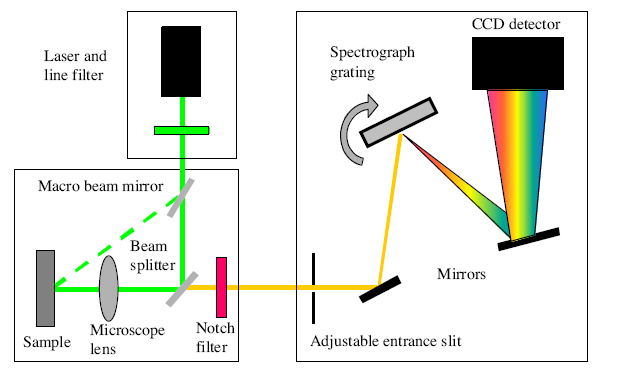
\includegraphics[scale=0.7]{Methodology/RamanSetup.png}
		\caption{A typical Raman spectroscope setup. Reproduced from www.sas.upenn.edu}
		\label{fig:MethodologyRamanSetup}
	\end{center}
\end{figure}

A Raman spectrometer used in this work is a Renishaw Raman spectrometer. The 532nm laser was used as a light source in a backscattering geometry. Unless otherwise specified the measurements were taken at room temperature and ambient pressure. An objective lens of 100x with 0.9 numerical aperture was used as the focusing lens. The laser power was set to be 1.6mW with 0.1s acquisition time for mapping and 1s acquisition time for single spectra. The grating of 1800 lines/mm was used resulting in a resolution of about 1.5 $cm^{-1}$. For calibration purposes a silicon sample was used with a peak at 520 $cm^{-1}$. All data analysis was performed using MATLAB software as described in chapter \ref{sec:MATLAB}.

\section{Photoluminescence spectroscopy}

The photoluminescence spectroscopy (PL) is an another versatile non-destructive characterisation technique. When applied to the 2D TMDCs it can provide great insight into the crystal stricture, electronic structure of the material as well as some direct information about its optical properties. One of the great advantages of PL spectroscopy is shared with the Raman spectroscopy in that the sample preparation and handling is very easy and quick allowing for high throughput of characterisation. Unlike Raman spectroscopy a substrate choice might become more important for PL measurements owing to the fact that the conductive substrate might result in PL quenching. Since the bandgap of many of the 2D TMDCs lies within the optical range of the spectrum or near to it a single laser at 532 nm can be used to excite the samples.

Photoluminescence is a type of luminescence where an excitation is provided by the incident light. In a semiconducting material like many of the 2D 2H TMDCs the electron from valence band is excited to the conduction band. Following the excitation the electron and resulting hole relax in both energy and momentum to the edge of the conduction and valence band respectively. Thus they form an exciton, a quasi particle that contains no net charge and can move across the material. An exciton in TMDCs can approach large sizes (Wannier-Mott exciton) due to great value of dielectric constant and resulting screening between the electron and the hole. Such exciton can also interact with the material by getting pinned by defect sites. After very short lifetime the exciton recombines emitting the photon at the same time. The photons emitted by the recombining exciton can be then collected. A plot of the photon count versus the energy of the detected photon forms the PL spectrum.

Therefore the PL spectrum can be used to directly infer the optical bandgap which is the electronic band gap of the material minus the binding energy of the exciton. In TMDCs on top of excitons additional type of quasi particle like trions or biexcitons can be found. Those particles exhibit varying level of binding energy and sometimes require special conditions to become excited. The PL spectrum can be therefore used to infer about the presence of those particles and therefore gain insight into the structure of the material. An energy diagram representing the photoluminescence process can be seen in Figure \ref{fig:MethodologyPLDiagram}.

\begin{figure}[!ht]
	\begin{center}
		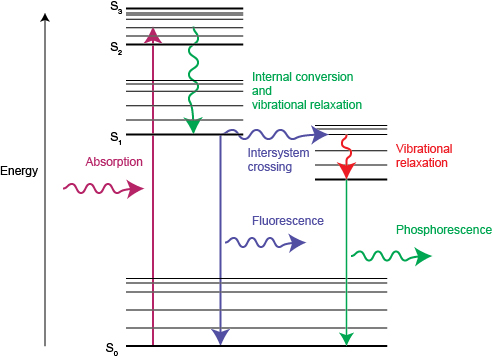
\includegraphics[scale=0.7]{Methodology/PLDiagram.png}
		\caption{The photoluminescence process.}
		\label{fig:MethodologyPLDiagram}
	\end{center}
\end{figure}

The PL signal becomes broadened due to variety of factors. On of the most important contributors is temperature which results in Gaussian broadening. At room temperature there is a constant peak broadening of about 25 meV. Because that broadening is relatively close to the binding energy of the trion ($\sim$30 meV). Therefore at room temperature the trion peak which is generally weaker than the exciton peak cannot be easily resolved. In order to be able to resolve those peaks a PL measurement at lower temperature can be performed.

A photoluminescence setup can look very similar to that of the Raman setup as seen in Figure \ref{fig:MethodologyRamanSetup}. A monochromatic light source e.g. a laser illuminates the sample at the energy greater than that of the materials bandgap. As a result of that the photons emitted from the material together with the inelastically (Raman) and elastically (Rayleigh) scattered photons pass through a filter to remove the latter. The remaining light is then passed through monochromator and detected at the CCD detector. As a result the PL and Raman spectra can be observed in the same spectrum, provided that the sample material can produce both of those signals. 

For low temperature (77K) measurements an environmental stage, Linkam THMS-350V. A pump was used to lower the pressure in the chamber down to about $2 \times 10^{-3}$ mbar. The liquid nitrogen was used to cool down the stage down to 77K. The stage was placed in Renishaw Raman spectrometer to capture PL spectra.

The PL spectrometer used in this work is a Renishaw Raman spectrometer. The 532nm green laser with objective lens of 100x with 0.9 numerical aperture was used and the data was recorded in backscattering configuration. The laser power used was 0.32mW with 0.1s exposition time for maps and up to 5s exposition time for a single extended spectrum. The 1800 lines/mm grating was used resulting in a resolution of about 0.2 meV. The spectrum was calibrated using silicon Raman peak at 520 $cm^{-1}$. All data analysis was carried out was done using MATLAB software as described in chapter \ref{sec:MATLAB}.

\section{X-ray photoelectron spectroscopy}

One of the most useful characterisation techniques for study of 2D TMDCs is X-ray photoelectron spectroscopy. It is a non-destructive method which allows to gain information about the chemical composition of the studied material. It is a very surface sensitive method that allows for obtaining signals from about 10 nm of the sample depth. In order to perform the XPS measurement the sample must be placed in high vacuum (about $10^{-8}$ mbar). It is therefore necessary that the sample contains no liquids or adsorbed gasses which would increase the pressure inside the analysis chamber. 

When a sample is irradiated with a beam of x-ray photons some of those photons get absorbed by the electrons in the sample. Because the energy of the incident photons is relatively large the electrons have enough energy to leave the atoms and travel towards the detector. At the detector their kinetic energy is measured. Because the energy of the incident x-ray photons is known and the kinetic energy of the photoelectrons is measured the remaining energy can be calculated using Equation \ref{eq:XPSEquation}:

\begin{equation}
E_{binding}  = E_{photon} - (E_{kinetic} + \Phi)
\label{eq:XPSEquation}
\end{equation}

If the $\Phi$ which is a instrumental correction factor is known then the $E_{binding}$ can be found. This binding energy depends on the specific atoms from which the electron as well as the specific atomic configuration. Because of that the chemical composition of a given sample surface can be determined. Additionally the number of detected electrons is directly correlated to the concentration of the atoms in the given sample the specific atomic percentages within the scanned area can be calculated. The number of detected electrons can be then plotted against the calculated corresponding binding energy of the electrons to form an XPS spectrum. A diagram of the XPS physics can be seen in Figure \ref{fig:MethodologyXPSSetup}.

In TMDCs the XPS can be used to determine the stoichiometric composition of the as grown material as well as detect any traces of unintentional doping from alkali or halogen atoms or intentional doping by e.g. In atoms. Additionally the amount of oxides as well as the presence of 2H or 1T phases can be quantitatively determined. 

The XPS spectra were collected using the Thermo Scientific K-Alpha XPS system. The Al $K_{\alpha}$ emission line was used as the x-ray source. The pass energy of 20 eV and the energy step of 0.1 eV were used. The XPS spectra were collected at room temperature and pressure of about $3 \times 10^{-8}$ mbar. The acquired data was analysed using Avantage software.

\begin{figure}[!ht]
	\begin{center}
		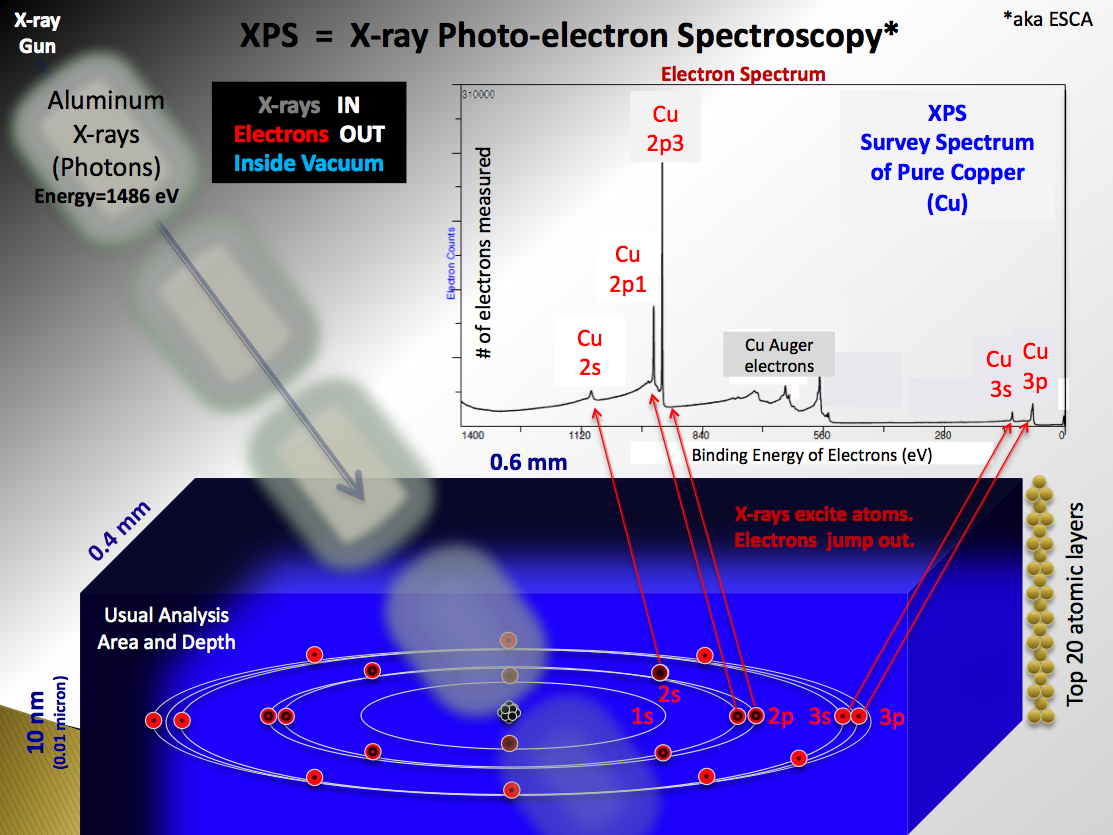
\includegraphics[scale=0.4]{Methodology/XPSSetup.png}
		\caption{Photoelectron effect energy diagram present during XPS.}
		\label{fig:MethodologyXPSSetup}
	\end{center}
\end{figure}

\section{Transfer}

Due to the nature of the 2D materials, the 2D TMDCs are generally always deposited on some substrate and cannot be used independently of it. Depending on the manufacturing method different substrates can be used to initially synthesise or deposit the material. In general however the initially used substrate is different to that which can be used for either characterisation or specific application. The samples synthesised by CVD are grown generally on $Si/SiO_2$ at very high temperature and as such cannot be readily used in electronic applications due to $Si$ deterioration at high temperature. To that effect the as grown samples are required to be transferred to a new substrate. 

In this work the wet transfer method has been utilised to transfer CVD grown samples from $Si/SiO_2$ to another $Si/SiO_2$, Au or TEM grid substrate. In this method the sample is first spin-coated with a thin layer of PMMA at 3000 RPM for 60 s. After that the sample is dried and heated up to about 50 {\degree}C for about 1 hour to ensure full polymerisation. Following that the substrate with the sample is then placed in a bath of 8\% KOH solution for about 45 min or until the $Si$ under the $SiO_2$ has completely sank to the bottom of the beaker. The thin layer of PMMA with the sample at the bottom is then scooped up with a glass slide and transferred to a DI water to remove the KOH. The sample is held in a water bath for about 30 min and the step is repeated 2-3 more times. After the last dilution step the sample is scooped onto a target substrate. The sample is then gently dried using compressed nitrogen or air to drive any water from between the PMMA and the substrate. The substrate is then heated up to about 50 {\degree}C for about an 1h to completely dry the sample of any water and ensure better adhesion to the substrate. The substrate is then placed in a bath of acetone and isopropanol heated up to 60 {\degree}C for about an 1h to remove the PMMA layer. After all PMMA has been removed the sample is heated again on a hot plate up to 100 {\degree}C to remove any traces of PMMA.

\section{Device fabrication}

The devices were prepared by collaborators from Exeter University: Iddo Amit, Gareth F. Jones, Jake D. Mehew, Agnes Bacon. In order to measure the electric properties of the as-grown materials the material can be used to make a field effect transistor (FET) device. For that purpose the as grown mono- and bi-layer $WS_2$ was transferred onto a $Si/SiO_2$ substrate with the $SiO_2$ layer of 285 nm in thickness. The $Si$, which is highly p-doped, then acts as a global gate electrode while the $SiO_2$ is a gate dielectric. On top of the deposited contacts for source and drain electrodes additional probes were used in each of the FET devices to eliminate any voltage contributions from the contacts and thus allow for correct measurement of the channel conductance. The drain and source drains as well as the voltage drains were deposited using electron beam lithography. The contacts as well as the probes were made using 50 nm thick Au, while the rest of the leads were made using 5nm thick Ti and 50 nm thick Au. Following the contacts and leads deposition the FET devices were annealed at 200 {\degree}C fpr 2h under $H_2/Ar$ (10/90) flow at 1 bar to remove any remaining PMMA from the lithographic process. The sample was then annealed at 115 {\degree}C for 60 h under high vacuum ($10^{-6}$ mbar) to remove any remaining water.

Following the FET preparation the samples were then characterised in a vacuum chamber in high vacuum ($10^{-6}$ mbar). A low noise source-meter was used to bias the drain electrode with source being grounded. Additionally another source was used to bias the gate electrode. The current across the channel $I_(ds)$ was measured using ammeter while the voltage $V_{A-B}$ across the voltage probes was measured with a voltmeter. The gate bias was applied until the measured current reached linear regime where it is described by Equation \ref{eq:FETCurrent} \cite{Sze2006}: 

\begin{equation}
I_d = {\mu}_nC_{Ox}\frac{W}{L}(V_{gs} - V_{th})V_{ds}
\label{eq:FETCurrent}
\end{equation}

where ${\mu}_n$ is electron field effect mobility, $C_{Ox}$ is the $SiO_2$ capacitance, W, L are the channel width and length, $V_{th}$ is the threshold voltage, $V_{ds}$ and $V_{gs}$ are the drain-source voltage and gain-source voltage respectively. From the measurement of the current the field-effect mobility for the mono- and bi-layer of the $WS_2$ can be calculated using the linear part of the plot from Equation \ref{eq:FETMobility}: 

\begin{equation}
\mu_{n} = C_{Ox}^{-1}\frac{d{\sigma}}{dV_{gs}}
\label{eq:FETMobility}
\end{equation}

where $\sigma$ is the channel conductivity which can be calculated from Equation \ref{eq:FETConductivity}:

\begin{equation}
\sigma = \frac{LI_{ds}}{W V_{A-B}}
\label{eq:FETConductivity}
\end{equation}

and the oxide capacitance $C_{Ox}$ was calculated to be 115$\mu F m^{-2}$ using Equation \ref{eq:FETCapacitance}:

\begin{equation}
C_{Ox} = \frac{{\epsilon}_0{\epsilon}_r}{d_{Ox}}
\label{eq:FETCapacitance}
\end{equation}

where ${\epsilon}_0$ and ${\epsilon}_r$ are the vacuum and relative permittivity of $SiO_2$ respectively and $d_{Ox}$ is the oxide thickness \cite{Sze2006}.

Additionally the the resistance vs temperature measurements were performed flakes were contacted using two wires configuration. The contacts were deposited using standard photolithographic method by applying the photo resist mask (AZ 5214E) followed by evaporation of Ti (5 nm) and Au (30 nm) using thermal evaporation and sputtering respectively. The measurements were then performed using six arm cryogenic probe station. The measurements were taken at high vacuum of $10^{-5}$ mbar and liquid nitrogen temperature. Following the measurements the conductivity was calculated from $\sigma = \frac{L}{RA}$, where L is the distance between contacts ($\sim$3 $\mu m$), R is the resistance while A is the flake cross section (0.9 nm - 40$\mu m$). The Keithley 2410 source measure unit as well as Lakeshor temperature controller were used for the measurement.

\section{Scanning electron microscopy (SEM)}

Scanning electron microscopy (SEM) is a versatile technique that allows for high resolution imaging of the sample surface. The fundamental operation of the SEM is based on a high energy (1 - 30 keV) electron beam which is rastered across the surface sample under high vacuum ($<10^{-5}$ mbar). The incident beam then is scattered by the atoms producing backscattered electrons, secondary electrons, Auger electrons, characteristic x-rays, fluorescent x-rays and continuum x-ray. The backscattered electrons (BSE) are those electrons that undergo elastic scattering during the process and are then measured by the detector. Similarly the secondary electrons (SE) are those electrons that undergo the inelastic scattering and can then, using a different detector to the BSE, can be detected and counted. The depth from which the BSE are detected ranges up to $\sim$100 nm while that of the SE is limited to $\sim$10 nm.

The SEM images were produced using field emission gun SEM (FEG-SEM, Gemini 1525) with an In-Lens SE detector. The FEG-SEM allows for narrower spot size ($<5 nm$) and a higher signal to noise ratio compared to the conventional thermionic emitters utilised in SEM \cite{Ogura2009}. Due to the thickness of the $WS_2$ the SE were primarily used for imaging. Due to the position of the In-Lens SE detector in the electron column with a rotational symmetry around the optical axis it allows for use of low energy ($\sim$1 - 5 keV) for acceleration and close distance. Because of that the contrast between different number of layers can be achieved for some 2D materials \cite{Kochat2011}. However in order to maintain good signal to noise ratio a slightly higher energy (5 - 10 keV) was utilised.

\begin{figure}[!ht]
	\begin{center}
		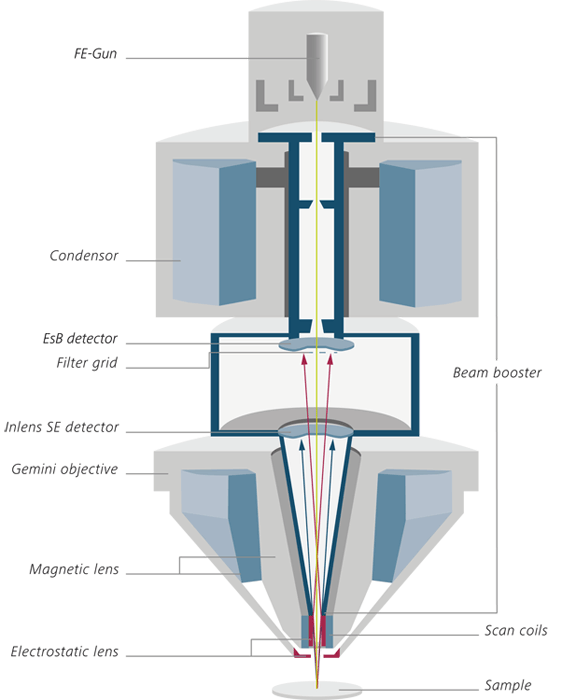
\includegraphics[scale=0.3]{Methodology/SEMSetup.png}
		\caption{Cross section of the SEM optical column. Reproduced from zeiss.com}
		\label{fig:MethodologySEMSetup}
	\end{center}
\end{figure}

\section{Atomic force microscopy (AFM)}

The atomic force microscopy (AFM) is one of scanning probe microscopy methods that allows for imaging surface morphology below the nm range as well as manipulation and force measurement. As seen in Figure \ref{fig:MethodologyAFMSetup} the AFM operates by touching and following the sample surface. The probe, which is a very sharply ended tip made of silicon or silicon nitride and a tip radius in the range of nanometers, is mounted on a cantilever. That cantilever is then controlled by a piezoelectric actuator which adjust the position based on the feedback from the laser measuring the actual cantilever deflection. The tip itself when brought close to the surface of the sample experiences a number of possible forces such as van der Waals forces, electrostatic forces, magnetic forces, chemical bond forces or mechanical contact forces which leads to a deflection one way or the other.

\begin{figure}[!ht]
	\begin{center}
		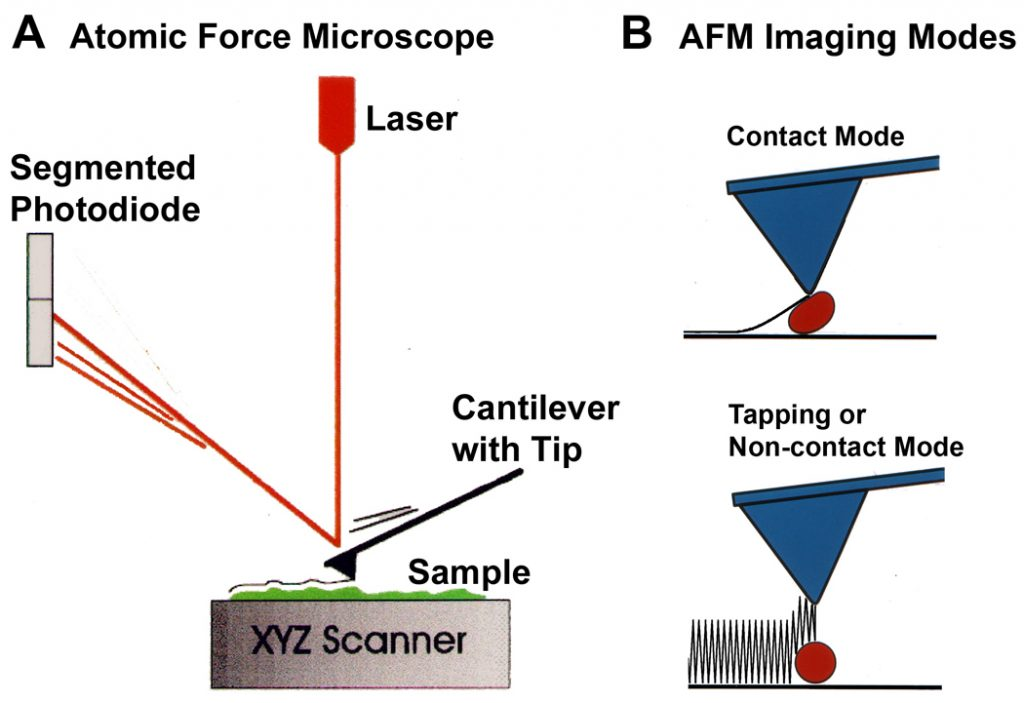
\includegraphics[scale=0.3]{Methodology/AFMSetup.png}
		\caption{Diagram of AFM setup and operating basics. Reproduced from ccem.mcmaster.ca}
		\label{fig:MethodologyAFMSetup}
	\end{center}
\end{figure}

The measurement can be performed in different modes as seen in Figure \ref{fig:MethodologyAFMSetup}. In contact mode the tip is dragged along the surface and either a tip deflection is directly measured or a constant height is maintained while the deflection required to maintain it is recorded \cite{Binnig1993}. Alternatively in a tapping mode the tip is oscillated at a resonant frequency and a constant amplitude is maintained. As the tip gets closer to the surface the forces act stronger and therefore the required correction is recorded and surface morphology and force can be determined. A tapping mode tends to be more useful for characterisation of 2D materials as it avoids damage to them but it is slower and may result in some artefacts \cite{Schmitz1997}.

When using tip with radius of $<$5 nm of curvature a lateral resolution of $\sim$5 nm and a vertical resolution of few \r{A} can be achieved. With a contaminated surface the resolution can quickly become bigger and therefore the thickness measurement of the 2D materials can become overestimated. In this work the measurements were carried out using AFM Asylum MFP 3D in a tapping mode with a probe tip made of silicon nitride and a radius of $\sim$8 nm on a PPP-NCHR 20 Nanosensors cantilever.

\section{TEM}

Transmission electron microscopy (TEM) is a microscopy technique in which a high energy (60-300 kV) electron beam is directed at a very thin ($<$100 nm) sample. As a result an image of the sample can be produced at resolution much greater than that achieved with optical microscopy due to much smaller wavelength of the electrons compared to the visible photons. As the electron beam passes through the sample it carries information about its electron density, periodicity and phase and can then form an image on a fluorescent screen. The resulting bright field image shows contrast due to variation in thickness across the sample, and as the magnification increases the interaction between the electron beam and the sample becomes more complex giving rise to different types of contrast. 

\begin{figure}[!ht]
	\begin{center}
		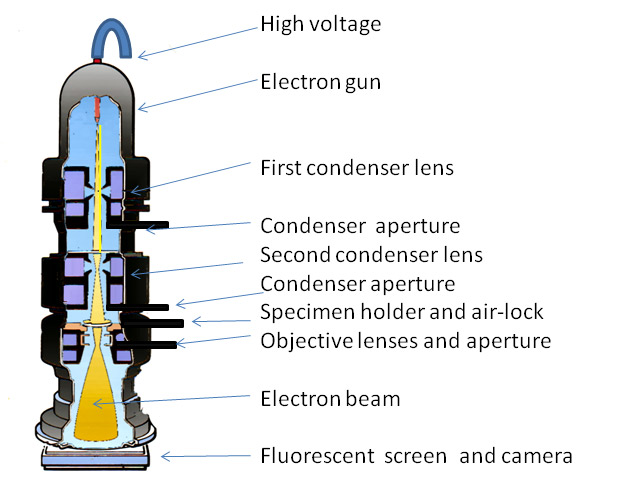
\includegraphics[scale=0.3]{Methodology/TEMSetup.png}
		\caption{Crossection of a TEM column. Reproduced from ccber.ucsb.edu}
		\label{fig:MethodologyTEMSetup}
	\end{center}
\end{figure}

Because the wavelength of the high energy electrons is much smaller than the distance between the atoms in a crystal lattice, the sample can act as a diffraction grating for the incident beam. By shifting the back focal plane instead of the image plane onto the imaging screen and inserting an aperture the diffraction pattern from selected area (SADP) can be achieved. This allows to gain information about the crystal structure and defects within much smaller area than what is possible with x-ray diffraction.

In this work the TEM used was a FEI Titan 80-300 S/TEM at 80kV with a monochromator and $C_s$ aberration image corrector. The focal series images were produced using different objective lens focus values ($C_s = -4\mu m$). Exit wave reconstruction was achieved using TrueImage (FEI).

\section{MATLAB Script}
\label{sec:MATLAB}
In order to analyse the PL and Raman spectra, both individual and maps, the MATLAB software was utilised. The spectra were exported from the Wire software used for Renishaw Raman spectrometer and they were then imported into MATLAB. Using "peakfit.m" script from "https://terpconnect.umd.edu/~toh/spectrum/peakfit.m" the peaks were fitted with required number of peaks. For peak fitting the Voigt peakshape was used. Several scripts were developed for the purpose of automating data import, analysis and peak fitting of PL and Raman maps.